%%%%%%%%%%%%%%%%%%%%%%%%%%%%%%%%%%%%%%%
\section{Communication model}
Since our system is highly interactive the communication model is very important. Figure~\ref{fig:dialogueDiagram} shows all the transaction that exist between the system and the user. Most transaction are pretty straight forward consisting of just some data being send from one to the other. The negotiate observable transaction is more complex and it therefore has its own flow control shown in figure~\ref{fig:trans3-control}. More details about these transactions are shown in tables TM-1 and TM-2.

\subsection{CRA communication plan}
\begin{figure}[htbp]
	\centering
		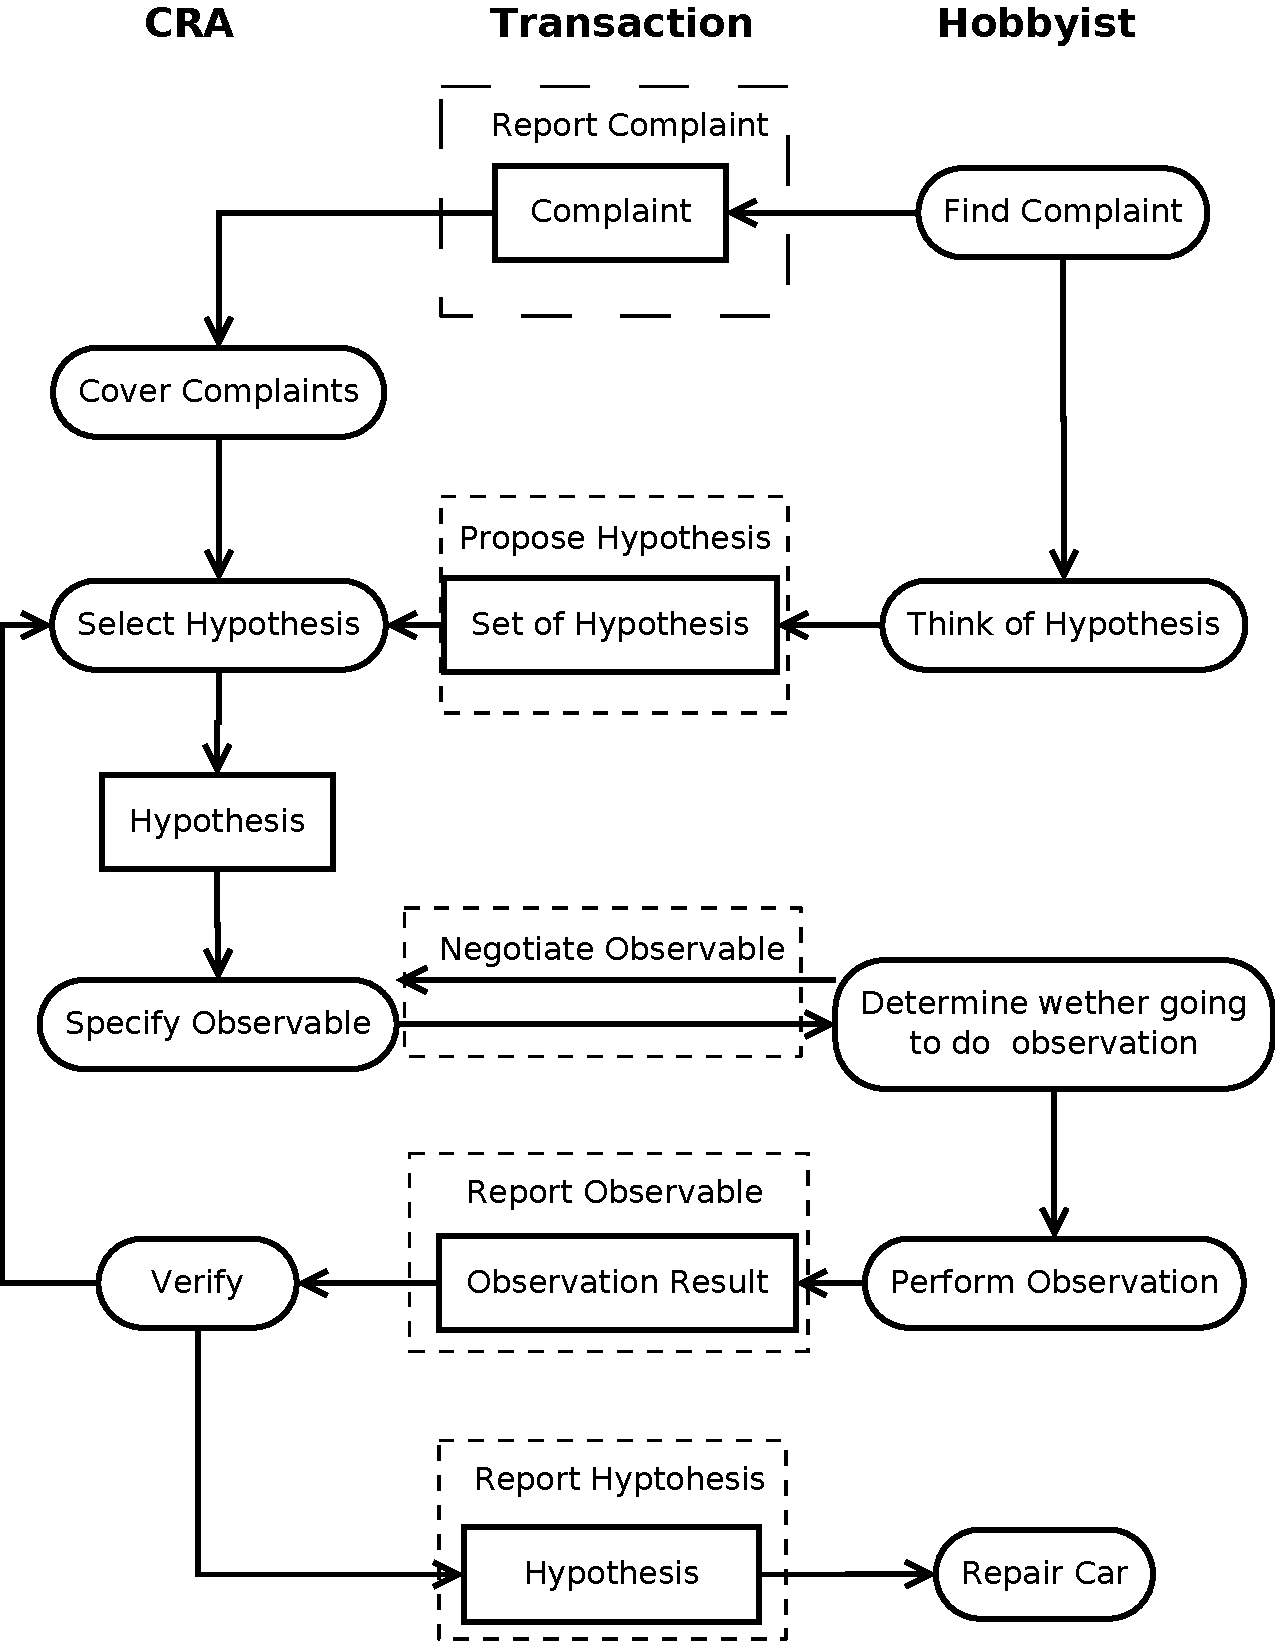
\includegraphics[width=1.00\textwidth]{dialogueDiagram.pdf}
	\caption{Dialogue diagram of the diagnoses task}
	\label{fig:dialogueDiagram}
\end{figure}

The control flow of the communication is shown in the communication plan (figure~\ref{fig:communicationPlan}). Because communication is so important in our system this plan is almost identical to the control flow of the CRA itself. 

As can be seen there is the need for a complaint at the start of the plan. Once this need is satisfied the state of the system will run in circles alternating between needing hypothesis, needing observables, found covering observations and observed observation until there are either no hypothesis or no observables left. At that point the plan is finished, either successful or unsuccessful.

\begin{figure}[htbp]
	\centering
		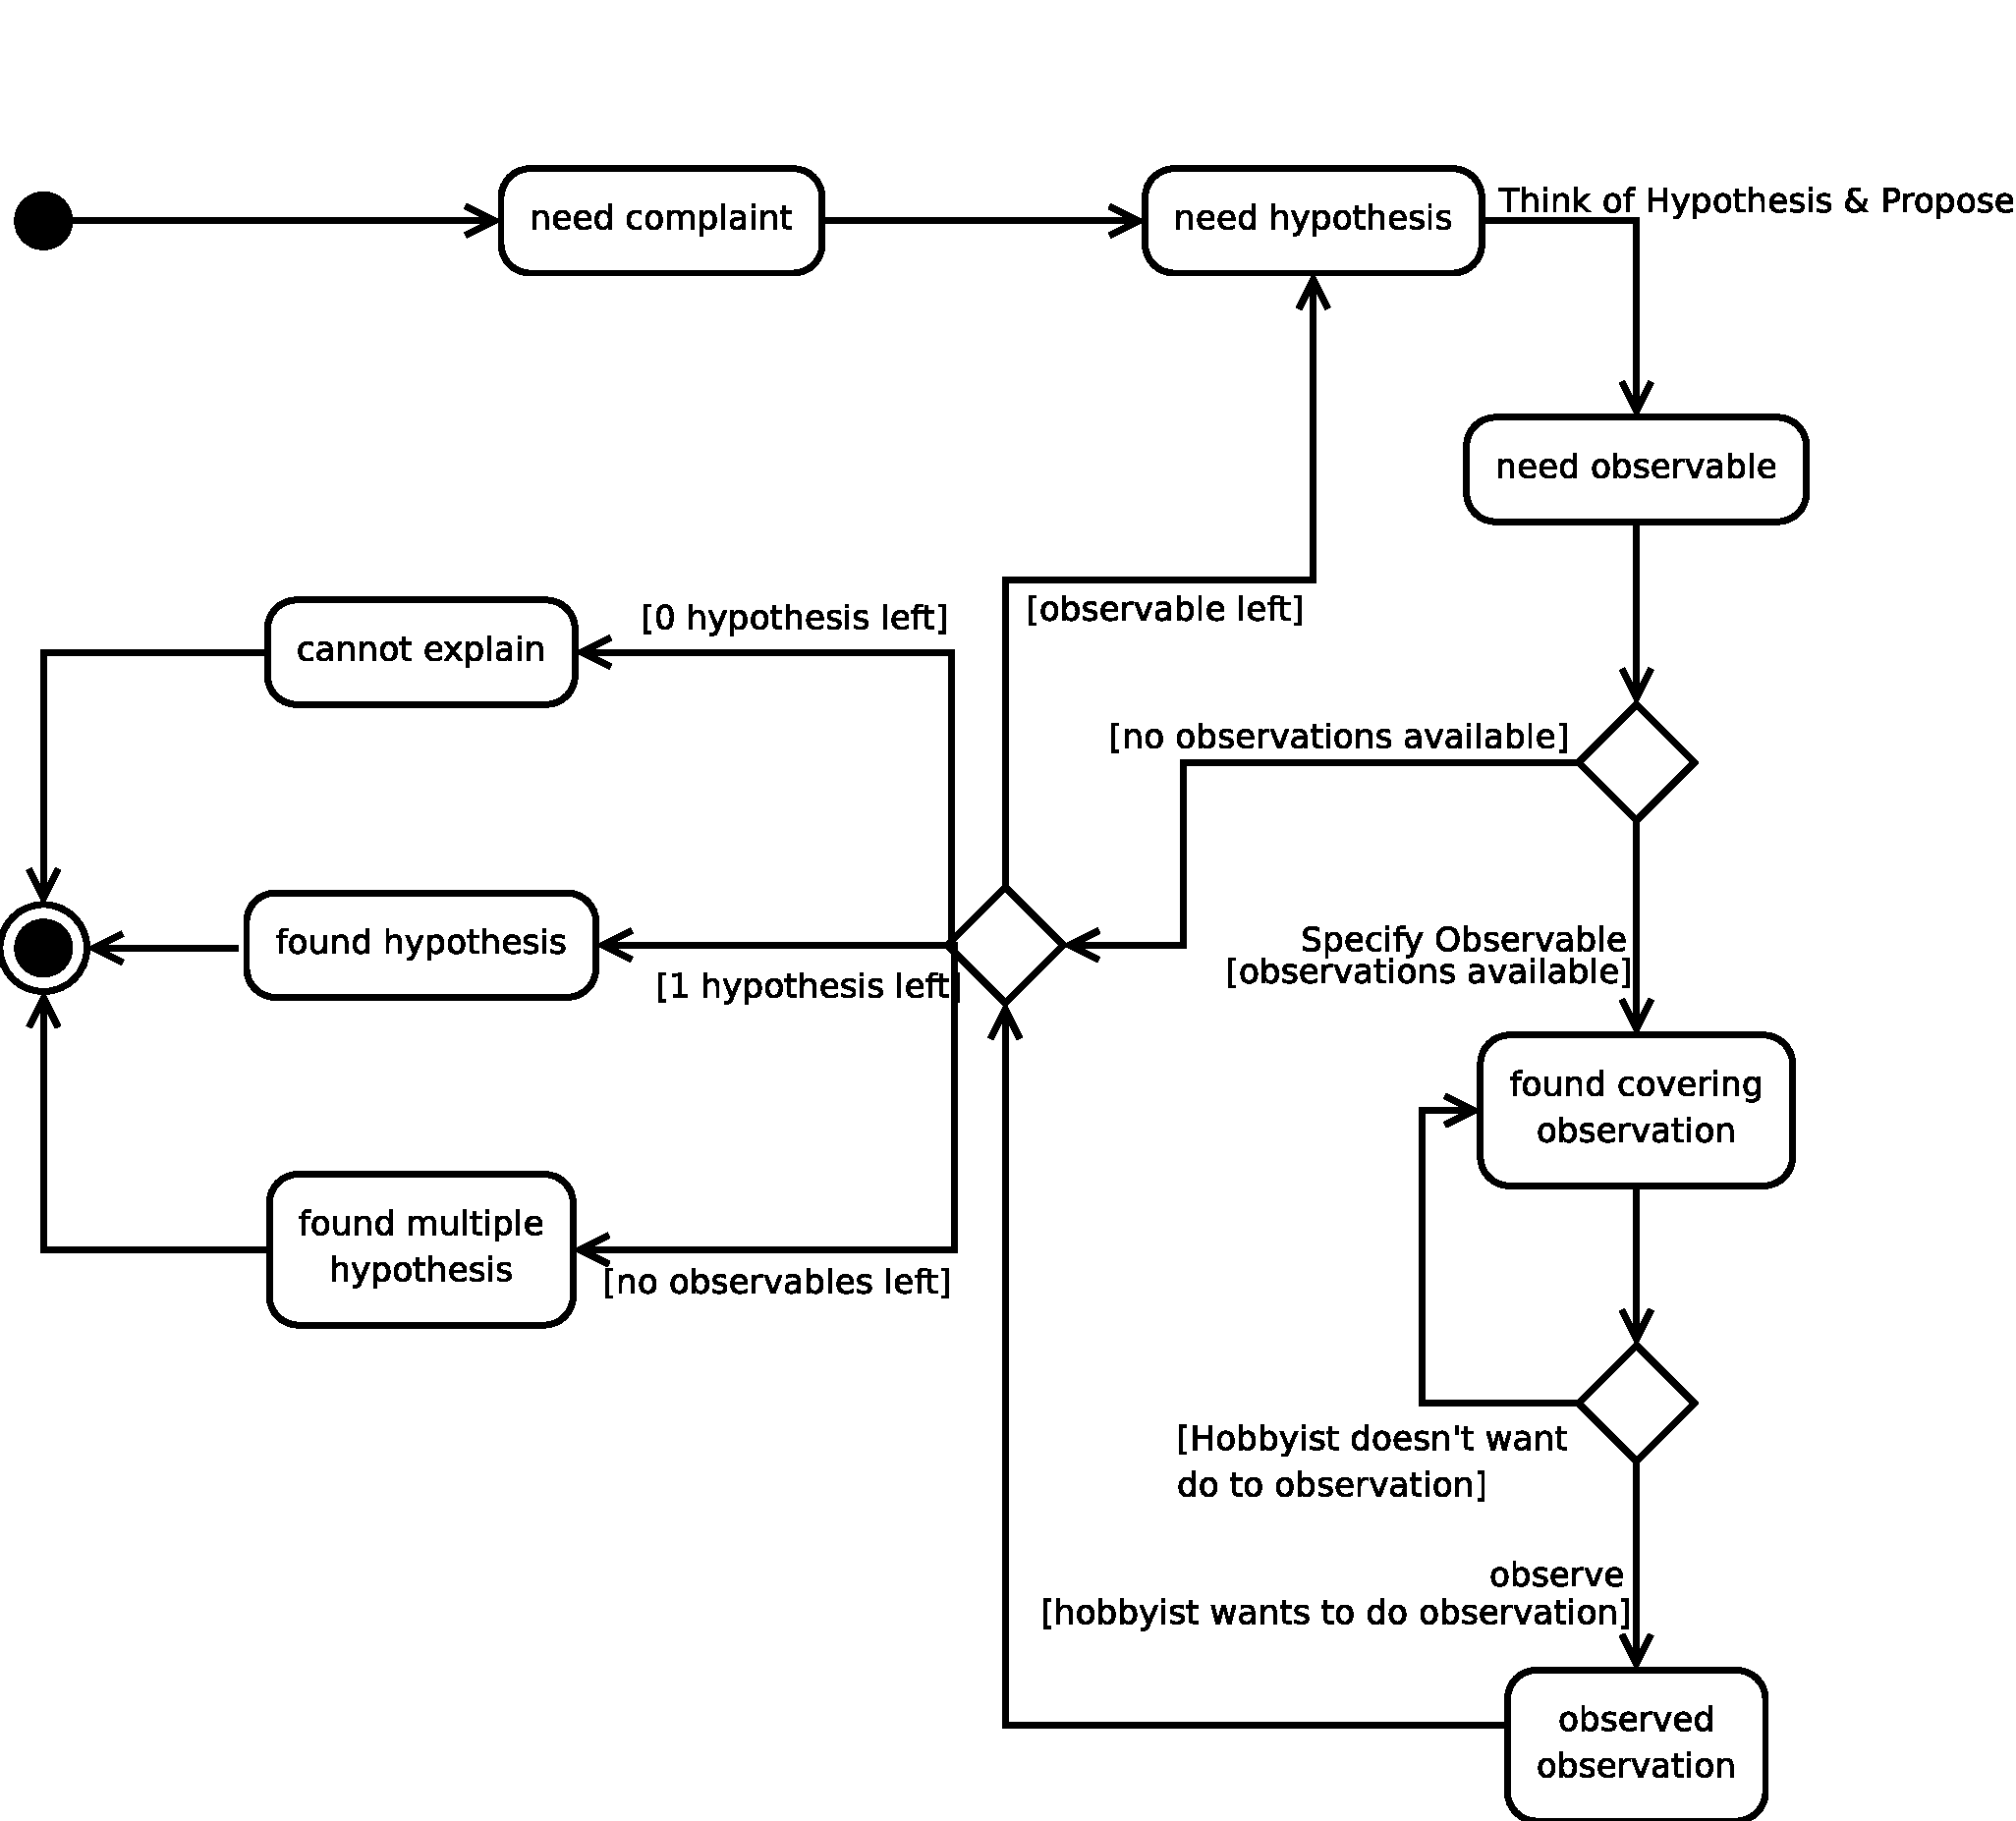
\includegraphics[width=1.00\textwidth]{communicationPlan.pdf}
	\caption{The communication plan of the diagnoses task.}
	\label{fig:communicationPlan}
\end{figure}

\subsection{CRA transactions}
% 1,2,5
\noindent
\begin{tabular}{%
       |>{\colleft}p{3cm}%
       |>{\colleft}p{8.5cm}|}
\hline
{\bf Communication model} &
   {\bf Transaction Description Worksheet CM-1} \\
\hline
\hline
\sc Transaction identifier/name &
	\emph{Transaction 1: Report complaint} \\

   %{\rm
   %A transaction is to be defined for each information object that is
   %output from some leaf task in the task model or in the knowledge
   %model (i.e., a transfer function), and that must be communicated to
   %another agent for use in its own tasks. The name must reflect, in a
   %user-understandable way, what is done with this information object
   %by the transaction. In addition to the name, give a brief
   %explanation here of the purpose of the transaction.
   %} 
\hline
\sc Information object &
	Transferring a complaint between the \emph{find complaint} and \emph{cover complaint} task. \\
   %{\rm
   %Indicate the (core) information object, and between which two
   %tasks it is to be transmitted.
   %} \\
\hline
\sc Agents involved &
	\emph{Car repair assistant}: receiving the complaint;\newline
	\emph{Hobbyist}: sending the complaint\\
   %{\rm
   %Indicate the agent that is sender of the information object,
   %and the agent that is receiving it.
   %} \\
\hline
\sc Communication plan &
	CRA communication plan\\

   %{\rm
   %Indicate the communication plan of which this transaction is a
   %component.
   %} \\
\hline
\sc Constraints &
	Before the transaction the car repair assistant must be ready to reiceve complaints\\

   %{\rm
   %Specify the requirements and (pre)conditions that must be fulfilled
   %so that the transaction can be carried out. Sometimes, it is also
   %useful to state post-conditions that are assumed to be valid after
   %the transaction.
   %} \\
\hline
\sc Information exchange specification &
	See worksheet CM-2 below.\\

   %{\rm
   %Transactions can have an internal structure, in that they consist
   %of several messages of different types, and/or handle additional
   %supporting information objects such as explanation or help items.
   %This is detailed in worksheet CM-2. At this point, only a reference
   %or pointer needs to be given to a later info exchange spec.
   %} \\
\hline
\end{tabular}


\noindent
\begin{tabular}{%
       |>{\colleft}p{3cm}%
       |>{\colleft}p{8.5cm}|}
\hline
{\bf Communication model} &
   {\bf Transaction Description Worksheet CM-1} \\
\hline
\hline
\sc Transaction identifier/name &
	\emph{Transaction 2: Propose hypothesis} \\

   %{\rm
   %A transaction is to be defined for each information object that is
   %output from some leaf task in the task model or in the knowledge
   %model (i.e., a transfer function), and that must be communicated to
   %another agent for use in its own tasks. The name must reflect, in a
   %user-understandable way, what is done with this information object
   %by the transaction. In addition to the name, give a brief
   %explanation here of the purpose of the transaction.
   %} 
\hline
\sc Information object &
	Transfering sets of hypothesis between the \emph{propose hypothesis} and \emph{select hypothesis} task. \\
   %{\rm
   %Indicate the (core) information object, and between which two
   %tasks it is to be transmitted.
   %} \\
\hline
\sc Agents involved &
	\emph{Hobbyist}: receiving the set of proposed hypothesis, sending a set of hypothesis (might be an empty set); \newline
	\emph{Car repair assistant}: sending a set of proposed hypothesis; receiving a set of hypothesis\\
   %{\rm
   %Indicate the agent that is sender of the information object,
   %and the agent that is receiving it.
   %} \\
\hline
\sc Communication plan &
	CRA communication plan\\

   %{\rm
   %Indicate the communication plan of which this transaction is a
   %component.
   %} \\
\hline
\sc Constraints &
	Before the transaction the car repair assistant must have a set of hypothesis ready. As a post condition one hypothesis has to be selected.\\

   %{\rm
   %Specify the requirements and (pre)conditions that must be fulfilled
   %so that the transaction can be carried out. Sometimes, it is also
   %useful to state post-conditions that are assumed to be valid after
   %the transaction.
   %} \\
\hline
\sc Information exchange specification &
	See worksheet CM-2 below.\\

   %{\rm
   %Transactions can have an internal structure, in that they consist
   %of several messages of different types, and/or handle additional
   %supporting information objects such as explanation or help items.
   %This is detailed in worksheet CM-2. At this point, only a reference
   %or pointer needs to be given to a later info exchange spec.
   %} \\
\hline
\end{tabular}

\noindent
\begin{tabular}{%
       |>{\colleft}p{3cm}%
       |>{\colleft}p{8.5cm}|}
\hline
{\bf Communication model} &
   {\bf Transaction Description Worksheet CM-1} \\
\hline
\hline
\sc Transaction identifier/name &
	\emph{Transaction 3: Negotiate observable} \\

   %{\rm
   %A transaction is to be defined for each information object that is
   %output from some leaf task in the task model or in the knowledge
   %model (i.e., a transfer function), and that must be communicated to
   %another agent for use in its own tasks. The name must reflect, in a
   %user-understandable way, what is done with this information object
   %by the transaction. In addition to the name, give a brief
   %explanation here of the purpose of the transaction.
   %} 
\hline
\sc Information object &
	Transferring observation instructions between the \emph{specify observable} and \emph{determine whether going to do observation} task. \\
   %{\rm
   %Indicate the (core) information object, and between which two
   %tasks it is to be transmitted.
   %} \\
\hline
\sc Agents involved &
	\emph{Car repair assistant}: sending observation instructions;\newline
	\emph{Hobbyist}: receiving observation instructions\\
   %{\rm
   %Indicate the agent that is sender of the information object,
   %and the agent that is receiving it.
   %} \\
\hline
\sc Communication plan &
	CRA communication plan\\

   %{\rm
   %Indicate the communication plan of which this transaction is a
   %component.
   %} \\
\hline
\sc Constraints &
	Before the transaction the car repair assistant must have a set of observables ready. As a post condition one observable must be excepted.\\

   %{\rm
   %Specify the requirements and (pre)conditions that must be fulfilled
   %so that the transaction can be carried out. Sometimes, it is also
   %useful to state post-conditions that are assumed to be valid after
   %the transaction.
   %} \\
\hline
\sc Information exchange specification &
	See worksheet CM-2 below.\\

   %{\rm
   %Transactions can have an internal structure, in that they consist
   %of several messages of different types, and/or handle additional
   %supporting information objects such as explanation or help items.
   %This is detailed in worksheet CM-2. At this point, only a reference
   %or pointer needs to be given to a later info exchange spec.
   %} \\
\hline
\end{tabular}


\noindent
\begin{tabular}{%
       |>{\colleft}p{3cm}%
       |>{\colleft}p{8.5cm}|}
\hline
{\bf Communication model} &
   {\bf Transaction Description Worksheet CM-1} \\
\hline
\hline
\sc Transaction identifier/name &
	\emph{Transaction 4: Report observable} \\

   %{\rm
   %A transaction is to be defined for each information object that is
   %output from some leaf task in the task model or in the knowledge
   %model (i.e., a transfer function), and that must be communicated to
   %another agent for use in its own tasks. The name must reflect, in a
   %user-understandable way, what is done with this information object
   %by the transaction. In addition to the name, give a brief
   %explanation here of the purpose of the transaction.
   %} 
\hline
\sc Information object &
	Transferring observation result between the \emph{perform observation} and \emph{verify} task. \\
   %{\rm
   %Indicate the (core) information object, and between which two
   %tasks it is to be transmitted.
   %} \\
\hline
\sc Agents involved &
	\emph{Hobbyist}: sending observation result;			\newline
	\emph{Car repair assistant}: receiving observation result	\\
   %{\rm
   %Indicate the agent that is sender of the information object,
   %and the agent that is receiving it.
   %} \\
\hline
\sc Communication plan &
	CRA communication plan\\

   %{\rm
   %Indicate the communication plan of which this transaction is a
   %component.
   %} \\
\hline
\sc Constraints &
	Before the transaction the hobbyist must have carried out the observation instructions and remembered there results.\\
   %{\rm
   %Specify the requirements and (pre)conditions that must be fulfilled
   %so that the transaction can be carried out. Sometimes, it is also
   %useful to state post-conditions that are assumed to be valid after
   %the transaction.
   %} \\
\hline
\sc Information exchange specification &
	See worksheet CM-2 below.\\

   %{\rm
   %Transactions can have an internal structure, in that they consist
   %of several messages of different types, and/or handle additional
   %supporting information objects such as explanation or help items.
   %This is detailed in worksheet CM-2. At this point, only a reference
   %or pointer needs to be given to a later info exchange spec.
   %} \\
\hline
\end{tabular}

\noindent
\begin{tabular}{|>{\colleft}p{3cm}|>{\colleft}p{8.5cm}|}
\hline
{\bf Communication model} &
   {\bf Transaction Description Worksheet CM-1} \\
\hline
\hline
\sc Transaction identifier/name &
	\emph{Transaction 5: Report hypothesis} \\

   %{\rm
   %A transaction is to be defined for each information object that is
   %output from some leaf task in the task model or in the knowledge
   %model (i.e., a transfer function), and that must be communicated to
   %another agent for use in its own tasks. The name must reflect, in a
   %user-understandable way, what is done with this information object
   %by the transaction. In addition to the name, give a brief
   %explanation here of the purpose of the transaction.
   %} 
\hline
\sc Information object &
	Transferring hypothesis result between the \emph{verify} and \emph{repair car} task. \\
   %{\rm
   %Indicate the (core) information object, and between which two
   %tasks it is to be transmitted.
   %} \\
\hline
\sc Agents involved &
	\emph{Car repair assistant}: sending hypothesis;	\newline
	\emph{Hobbyist}: receiving hypothesis			\\
   %{\rm
   %Indicate the agent that is sender of the information object,
   %and the agent that is receiving it.
   %} \\
\hline
\sc Communication plan &
	CRA communication plan\\

   %{\rm
   %Indicate the communication plan of which this transaction is a
   %component.
   %} \\
\hline
\sc Constraints &
	Before the transaction the car repair assistant must have either no observations left or he has one or less hypothesis left.\\
   %{\rm
   %Specify the requirements and (pre)conditions that must be fulfilled
   %so that the transaction can be carried out. Sometimes, it is also
   %useful to state post-conditions that are assumed to be valid after
   %the transaction.
   %} \\
\hline
\sc Information exchange specification &
	See worksheet CM-2 below.\\

   %{\rm
   %Transactions can have an internal structure, in that they consist
   %of several messages of different types, and/or handle additional
   %supporting information objects such as explanation or help items.
   %This is detailed in worksheet CM-2. At this point, only a reference
   %or pointer needs to be given to a later info exchange spec.
   %} \\
\hline
\end{tabular}
\noindent
\begin{tabular}{|>{\colleft}p{3cm}|>{\colleft}p{8.5cm}|} \hline
{\bf Communication model} 	& {\bf Information Exchange Specification Worksheet CM-2} \\ \hline \hline
\sc Transaction 			& \emph{Transaction 1: Report complaint}  \\ \hline
\sc Agents involved 		& 1. {\bf Sender}(Hobbyist): Initiate repair  \newline
					  2. {\bf Receiver}(Car repair assistant): Initiate repair \newline
					  3. {\bf Sender}(Car repair assistant): List of complaints  \newline
					  4. {\bf Receiver}(Hobbyist): List of complaints  \newline
					  5. {\bf Sender}(Hobbyist): Complaint  \newline
					  6. {\bf Receiver}(Car repair assistant): Complaint \\ \hline
\multicolumn{2}{|l|}{\textsc{Information items}} \\ \hline
   					%List all information items that are to be transmitted in this
   					%transaction. This includes the (`core') information object the
   					%transfer of which is the purpose of the transaction. However, it may contain
   					%other, supporting, information items, that, for example, provide help
   					%or explanation. For each information item, describe the following:
   
INITIATE REPAIR			&  1. {\bf Role}: A core information object. \newline
					% whether it is a {\em core} object, or a {\em support} item.
					   2. {\bf Form}: A signal indicating the start of a repair process \newline
					% the syntactic form in which it transmitted to another agent , e.g., data string, canned text, a certain type of diagram, 2D or 3D plot.
					   3. {\bf Medium}: By starting the program using an icon or command\\
					% the medium through which it is handled in the agent-agent interaction, e.g., a pop-up window, navigation and selection within a menu, command-line interface, human intervention.
LIST OF COMPLAINTS		&  1. {\bf Role}: A support information object. \newline
					   2. {\bf Form}: A list of strings \newline
					   3. {\bf Medium}: As menu items\\
COMPLAINT				&  1. {\bf Role}: A core information object. \newline
					   2. {\bf Form}: An identifier \newline
					   3. {\bf Medium}: As a selection within a menu\\ \hline
\multicolumn{2}{|l|}{\textsc{Message specifications}}\\ \hline
					% Describe all messages that make up the transaction. For each individual message describe:
INITIATION-MESSAGE		& {\bf Communication type}: ORDER\newline
					% the communication type of the message describing its intention (``illocutionary force,'' in speech-act terminology). 
					  {\bf Content}: Initiate repair\newline
					% the statement or proposition contained in the message.
					%&  3. {\bf Reference}: \\ \hline
					%in certain cases, it may be useful to add a reference to, for example, what domain knowledge model or agent capability is required to be able to send or process the message.
					  {\bf From}: Hobbyist\newline
					  {\bf To}: Car repair assistant\\
COMPLAINTS-LIST-MESSAGE		& {\bf Communication type}: REQUIRE\newline
					  {\bf Content}: List of complaints and the request to chose one\newline
					%&  3. {\bf Reference}: \newline
					  {\bf From}: Car repair assistant\newline
					  {\bf To}: Hobbyist\\
COMPLAINT-MESSAGE			& {\bf Communication type}: AGREE/REPORT\newline
					  {\bf Content}: Complaint\newline
					%&  3. {\bf Reference}: \\ \hline
					  {\bf From}: Hobbyist\newline
					  {\bf To}: Car repair assistant\\\hline
%\sc Control over messages 	& \\ \hline
   					%Give, if necessary, a control specification over the messages
   					%within the transaction. This can be done in pseudocode format or
   					%in a state-transition diagram, similar to how the control over
   					%transaction within the communication plan is specified. The
   					%difference is just the level of detail.
\end{tabular}

\noindent
\begin{tabular}{|>{\colleft}p{3cm}|>{\colleft}p{8.5cm}|} \hline
{\bf Communication model} 	& {\bf Information Exchange Specification Worksheet CM-2} \\ \hline \hline
\sc Transaction 			& \emph{Transaction 2: Propose hypothesis}  \\ \hline
\sc Agents involved 		& 1. {\bf Sender}(Car repair assistant): List of hypothesis  \newline
					  2. {\bf Receiver}(Hobbyist): List of hypothesis \newline
					  3. {\bf Sender}(Hobbyist): Hypothesis  \newline
					  4. {\bf Receiver}(Car repair assistant): Hypothesis \\ \hline
\multicolumn{2}{|l|}{\textsc{Information items}} \\ \hline
   					%List all information items that are to be transmitted in this
   					%transaction. This includes the (`core') information object the
   					%transfer of which is the purpose of the transaction. However, it may contain
   					%other, supporting, information items, that, for example, provide help
   					%or explanation. For each information item, describe the following:
LIST OF HYPOTHESIS		&  1. {\bf Role}: A support information object. \newline
					   2. {\bf Form}: A list of strings \newline
					   3. {\bf Medium}: As menu items\\
HYPOTHESIS				&  1. {\bf Role}: A core information object. \newline
					   2. {\bf Form}: An identifier \newline
					   3. {\bf Medium}: As a selection within a menu\\
\multicolumn{2}{|l|}{\textsc{Message specifications}}\\ \hline
					% Describe all messages that make up the transaction. For each individual message describe:
HYPOTHESIS-LIST-MESSAGE		& {\bf Communication type}: REQUIRE\newline
					  {\bf Content}: List of hypothesis and the request to chose one\newline
					%&  3. {\bf Reference}: \newline
					  {\bf From}: Car repair assistant\newline
					  {\bf To}: Hobbyist\\
HYPOTHESIS-MESSAGE		& {\bf Communication type}: AGREE/REPORT\newline
					  {\bf Content}: Hypothesis\newline
					%&  3. {\bf Reference}: \\ \hline
					  {\bf From}: Hobbyist\newline
					  {\bf To}: Car repair assistant\\
NO-HYPOTHESIS-MESSAGE		& {\bf Communication type}: REJECT-ta\newline
					  {\bf Content}: rejection \newline
					%&  3. {\bf Reference}: \\ \hline
					  {\bf From}: Hobbyist\newline
					  {\bf To}: Car repair assistant\\\hline
%\textsc{Control over messages}& See code below. \\ \hline
   					%Give, if necessary, a control specification over the messages
   					%within the transaction. This can be done in pseudocode format or
   					%in a state-transition diagram, similar to how the control over
   					%transaction within the communication plan is specified. The
   					%difference is just the level of detail.
\end{tabular}

%\begin{verbatim}
%SEND(COMPONENT-LIST-MESSAGE)
%REPEAT WHILE <no NO-HYPOTHESIS-MESSAGE received>
%  IF <user wants to suggest a hypothesis> 
%  THEN 
%    IF <COMPONENT-LIST-MESSAGE received> 
%    THEN 
%      SEND(COMPONENT-MESSAGE)
%    END-IF
%    IF <MALFUNCTION-LIST-MESSAGE received> 
%    THEN 
%      SEND(MALFUNCTION-MESSAGE)
%    END-IF
%  ELSE 
%    SEND NO-HYPOTHESIS-MESSAGE
%  END-IF
%  IF <COMPONENT-MESSAGE received>  
%  THEN 
%    SEND(MALFUNCTION-LIST-MESSAGE)
%  END-IF
%  IF <MALFUNCTION-MESSAGE received> 
%  THEN 
%    PROCESS(store-hypothesis)
%  END-IF
%END-REPEAT
%\end{verbatim}


\noindent
\begin{tabular}{ %
       |>{\colleft}p{4cm}%
       |>{\colleft}p{8.5cm}|}
\hline
{\bf Communication model} & {\bf Information Exchange Specification Worksheet CM-2} \\
\hline
\hline
{\sc Transaction} &
%   Give the transaction identifier and the name of which this information
%   exchange specification is a part.
Transaction 3: Negotiate Observable
 \\
\hline
{\sc Agents involved} &
1. {\bf Sender}
%agent sending the information item(s)
CRA send a request for an observation, and an explanation of that observation
\newline
2. {\bf Receiver}:
The hobbyist receives the request for an observation, and an explanation.
%agent receiving the information item(s)
\\
\hline
\multicolumn{2}{|l|}{\textsc{Information items}} \\ \hline
&  There are two information objects, the name of the observation to be done, and an
explanation of that observation. 
%   List all information items that are to be transmitted in this
%   transaction. This includes the (`core') information object the
%   transfer of which is the purpose of the transaction. However, it may contain
%   other, supporting, information items, that, for example, provide help
%   or explanation. For each information item, describe the following:
   \newline
  1. {\bf Role}: The name of the observation is core, while the explanation is
support.
%whether it is a core object, or a support item.
   \newline
  2. {\bf Form}: The name of the observation is a string. The explanation is
canned rich text.
     % the syntactic form in which it transmitted to
     % another agent , e.g., data string, canned text, a certain type of
     % diagram, 2D or 3D plot.
   \newline
  3. {\bf Medium}: The name of the observation can be selected in a menu. The
explanation can be shown in a text box.
     % the medium through which it is handled in the
     % agent-agent interaction, e.g., a pop-up window, navigation and
     % selection within a menu, command-line interface, human
     % intervention.
   \\
\hline
\multicolumn{2}{|l|}{\textsc{Message specifications}}\\ \hline
{\sc 1. REQUEST-OBSERVATION} &
   {\bf Communication type}: REQUEST \newline
   {\bf Content}: Request for some observation \newline
   {\bf From}: CRA \newline
   {\bf To}: The hobbyist \\
   
{\sc 2. OFFER-OBSERVATION} &
   {\bf Communication type}: OFFER \newline
   {\bf Content}: The Hobbyist wants to do a certain observation \newline
  {\bf From}: The hobbyist \newline
  {\bf To}: CRA \\
   
{\sc 3. DO-OBSERVATION} &
   {\bf Communication type}: ORDER \newline
  {\bf Content}: explanation and observation the hobbyist needs to make\newline
  {\bf From}: CRA \newline
  {\bf To}: The hobbyist \\
   
{\sc 4. REJECT-OBSERVATION-REQUEST} &
   {\bf Communication type}: REJECT-ta \newline
  {\bf Content}: Don't want to do this observation \newline
  {\bf From}: The hobbyist \newline
  {\bf To}: CRA \\
   
{\sc 5. REJECT-OBSERVATION-OFFER} &
   {\bf Communication type}: REJECT-td \newline
  {\bf Content}: Explanation why that observation is not needed \newline
  {\bf From}: CRA \newline
  {\bf To}: The hobbyist \\
   
\hline
\sc Control over messages &
    % Give, if necessary, a control specification over the messages
    % within the transaction. This can be done in pseudocode format or
    % in a state-transition diagram, similar to how the control over
    % transaction within the communication plan is specified. The
    % difference is just the level of detail.
    See figure~\ref{fig:trans3-control}.
   \\
\hline
\end{tabular}

\begin{figure}[htbp]
	\centering
		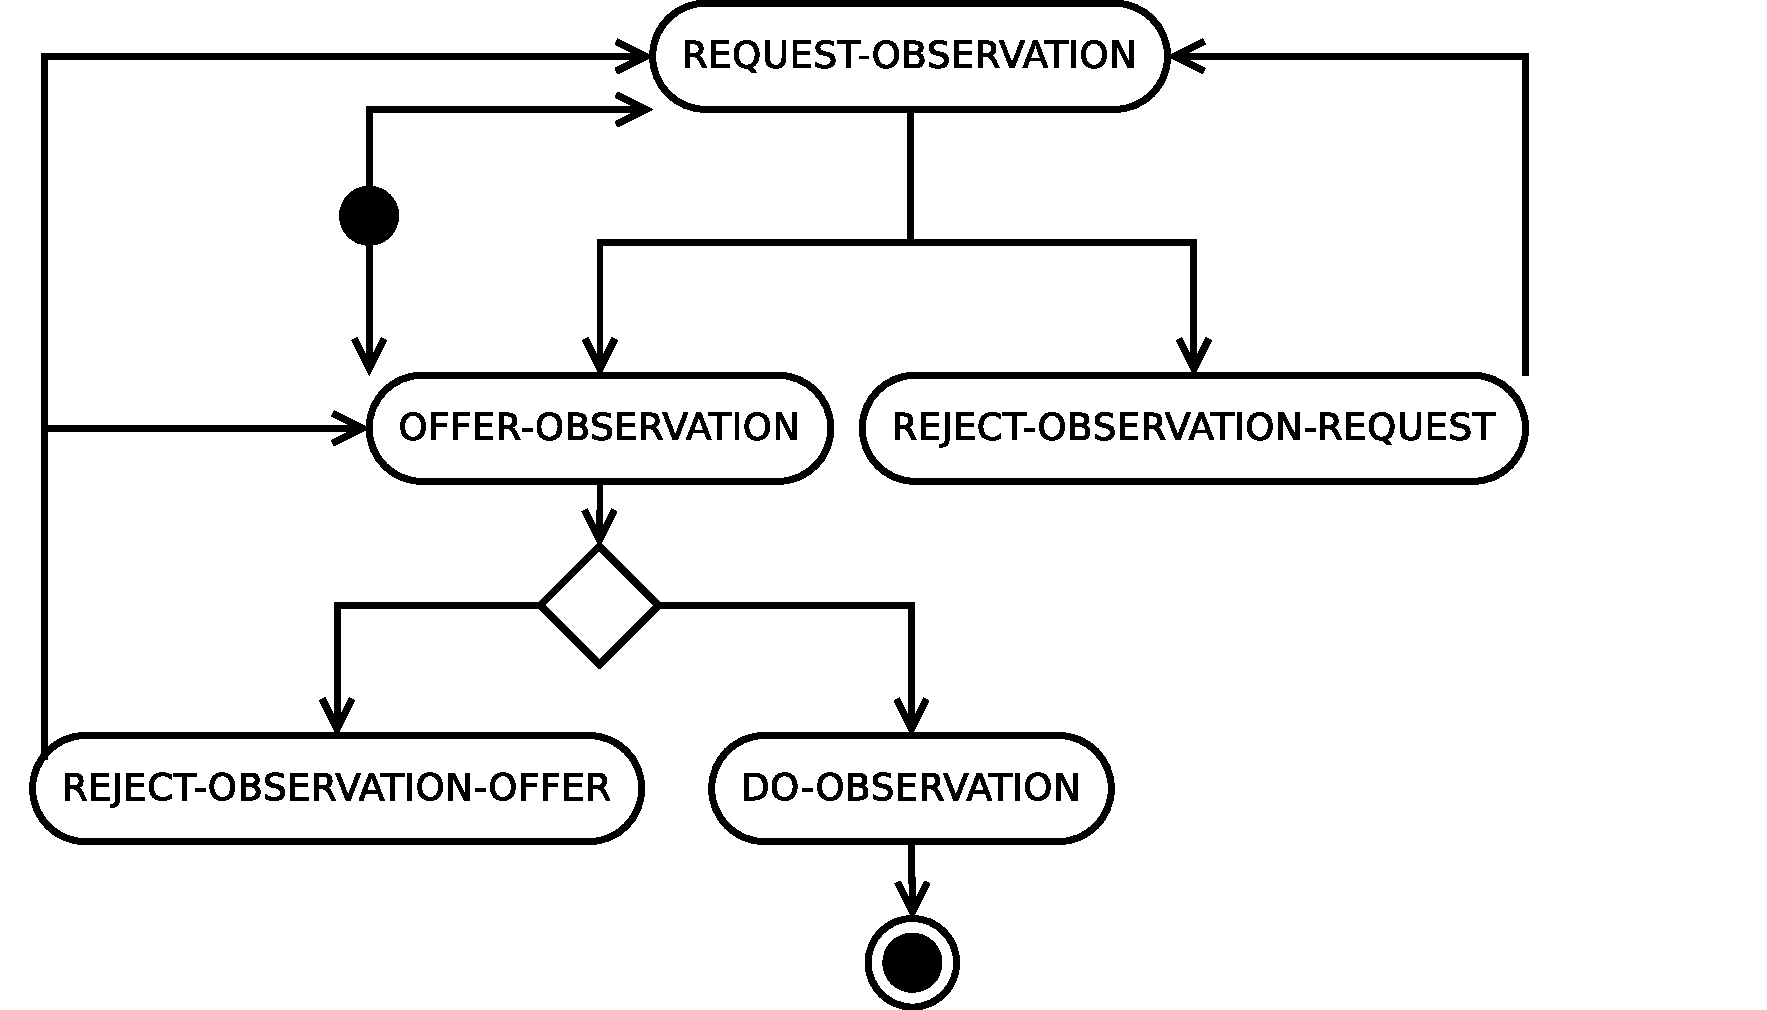
\includegraphics[width=1.00\textwidth]{trans3-control.pdf}
	\caption{Control flow of the negotiate observable transaction}
	\label{fig:trans3-control}
\end{figure}




\noindent
\begin{tabular}{|>{\colleft}p{3cm}|>{\colleft}p{8.5cm}|} \hline
{\bf Communication model} 	& {\bf Information Exchange Specification Worksheet CM-2} \\ \hline \hline
\sc Transaction 			& \emph{Transaction 4: Report observable} \\ \hline
\sc Agents involved 		& 1. {\bf Sender}(Car repair assistant): Observation result options  \newline
					  2. {\bf Receiver}(Hobbyist): Observation result options \newline
					  3. {\bf Sender}(Hobbyist): Observation result \newline
					  4. {\bf Receiver}(Car repair assistant): Observation result \\ \hline
					  
\multicolumn{2}{|l|}{\textsc{Information items}} \\ \hline
   					%List all information items that are to be transmitted in this
   					%transaction. This includes the (`core') information object the
   					%transfer of which is the purpose of the transaction. However, it may contain
   					%other, supporting, information items, that, for example, provide help
   					%or explanation. For each information item, describe the following:
OBSERVATION RESULT OPTIONS	&  1. {\bf Role}: A support information object. \newline
					% whether it is a {\em core} object, or a {\em support} item.
					   2. {\bf Form}: List of strings  \newline
					% the syntactic form in which it transmitted to another agent , e.g., data string, canned text, a certain type of diagram, 2D or 3D plot.
					   3. {\bf Medium}: Varies, it might be a menu or it might be a free form with suggestions noted separately\\ 
					% the medium through which it is handled in the agent-agent interaction, e.g., a pop-up window, navigation and selection within a menu, command-line interface, human intervention.
OBSERVATION RESULT		&  1. {\bf Role}: A core information object. \newline
					   2. {\bf Form}: Varies, it might be a identifier, a number or a string. \newline
					   3. {\bf Medium}: Varies, it might be selection in a menu or it might be typed in a field.\\ \hline
					
\multicolumn{2}{|l|}{\textsc{Message specifications}}\\ \hline
					% Describe all messages that make up the transaction. For each individual message describe:
OPTION-MESSAGE			& {\bf Communication type}: ASK \newline
					% the communication type of the message describing its intention (``illocutionary force,'' in speech-act terminology). 
					  {\bf Content}: Observation result options and the request to provide the actual observation result \newline
					% the statement or proposition contained in the message.
					% {\bf Reference}: car repair information\newline
					%in certain cases, it may be useful to add a reference to, for example, what domain knowledge model or agent capability is required to be able to send or process the message.
					  {\bf From}: Car repair assistant\newline
					  {\bf To}: Hobbyist\\ \hline
					  
OBSERVATION-MESSAGE		& {\bf Communication type}: REPLY \newline
					% the communication type of the message describing its intention (``illocutionary force,'' in speech-act terminology). 
					  {\bf Content}: The observation result \newline
					% the statement or proposition contained in the message.
					% {\bf Reference}: car repair information\newline
					%in certain cases, it may be useful to add a reference to, for example, what domain knowledge model or agent capability is required to be able to send or process the message.
					  {\bf From}: Hobbyist\newline
					  {\bf To}: Car repair assistant\\ \hline
%\sc Control over messages 	& \\ \hline
   					%Give, if necessary, a control specification over the messages
   					%within the transaction. This can be done in pseudocode format or
   					%in a state-transition diagram, similar to how the control over
   					%transaction within the communication plan is specified. The
   					%difference is just the level of detail.
\end{tabular}



\noindent
\begin{tabular}{|>{\colleft}p{3cm}|>{\colleft}p{8.5cm}|} \hline
{\bf Communication model} 	& {\bf Information Exchange Specification Worksheet CM-2} \\ \hline \hline
\sc Transaction 			& \emph{Transaction 5: Report hypothesis} \\ \hline
\sc Agents involved 		& 1. {\bf Sender}(Car repair assistant): Hypothesis  \newline
					  2. {\bf Sender}(Car repair assistant): Hypothesis argumentation \newline
					  3. {\bf Sender}(Car repair assistant): Repair plan \newline
					  4. {\bf Receiver}(Hobbyist): Hypothesis \newline
					  5. {\bf Receiver}(Hobbyist): Hypothesis argumentation \newline
					  6. {\bf Receiver}(Hobbyist): Repair plan \\ \hline
					  
\multicolumn{2}{|l|}{\textsc{Information items}} \\ \hline
   					%List all information items that are to be transmitted in this
   					%transaction. This includes the (`core') information object the
   					%transfer of which is the purpose of the transaction. However, it may contain
   					%other, supporting, information items, that, for example, provide help
   					%or explanation. For each information item, describe the following:
HYPOTHESIS				&  1. {\bf Role}: A core information object. \newline
					% whether it is a {\em core} object, or a {\em support} item.
					   2. {\bf Form}: A string stating the hypothesis \newline
					% the syntactic form in which it transmitted to another agent , e.g., data string, canned text, a certain type of diagram, 2D or 3D plot.
					   3. {\bf Medium}: Displayed in the main window\\ 
					% the medium through which it is handled in the agent-agent interaction, e.g., a pop-up window, navigation and selection within a menu, command-line interface, human intervention.
HYPOTHESIS ARGUMENTATION	&  1. {\bf Role}: A support information object. \newline
					   2. {\bf Form}: A list of strings each stating one reasoning step \newline
					   3. {\bf Medium}: Displayed in the main window\\
REPAIR PLAN				&  1. {\bf Role}: A support information object. \newline
					   2. {\bf Form}: A text, possibly with images\newline
					   3. {\bf Medium}: Displayed in the main window\\ \hline
					
\multicolumn{2}{|l|}{\textsc{Message specifications}}\\ \hline
					% Describe all messages that make up the transaction. For each individual message describe:
HYPOTHESIS-MESSAGE		& {\bf Communication type}: REPORT \newline
					% the communication type of the message describing its intention (``illocutionary force,'' in speech-act terminology). 
					  {\bf Content}: The hypothesis, the hypotheses argumentation and the repair plan (plan depending on car repair information)\newline
					% the statement or proposition contained in the message.
					  {\bf Reference}: car repair information\newline
					%in certain cases, it may be useful to add a reference to, for example, what domain knowledge model or agent capability is required to be able to send or process the message.
					  {\bf From}: Hobbyist\newline
					  {\bf To}: Car repair assistant\\ \hline
					  
%\sc Control over messages 	& \\ \hline
   					%Give, if necessary, a control specification over the messages
   					%within the transaction. This can be done in pseudocode format or
   					%in a state-transition diagram, similar to how the control over
   					%transaction within the communication plan is specified. The
   					%difference is just the level of detail.
\end{tabular}
